\documentclass[a4paper,12pt]{article}

\usepackage{authblk}
\usepackage[margin=1.5in]{geometry}
\usepackage{setspace}
\usepackage[T1]{fontenc}
\usepackage{calc}
\usepackage[hyphens]{url}

\usepackage{amsmath}

\usepackage[mono=false]{libertine}
\usepackage{unicode-math}
\setmathfont[Scale=MatchUppercase]{libertinusmath-regular.otf}

\usepackage{inconsolata}
%\usepackage{fontspec}
\setmonofont{inconsolata}

\usepackage{listings}
\lstset{language=R, keywordstyle=\color{black}, frameround=fttt, basicstyle=\ttfamily}

\usepackage{pifont}

\usepackage{hhline}
\usepackage{booktabs}
\usepackage{longtable}
\setlength{\LTleft}{0pt}
\usepackage{colortbl}
\usepackage{gb4e-}
\usepackage{graphicx}

\usepackage[backend=biber,
	natbib=true,
	style=bst/unified/bbx/biblatex-sp-unified,
	citestyle=bst/unified/cbx/sp-authoryear-comp,
	maxbibnames=99,
	isbn=false,
	doi=false,
	eprint=false
]{biblatex}

% \usepackage{fancyhdr}
% \pagestyle{fancy}

\newcommand{\Lf}{
  \setlength{\itemsep}{1pt}
  \setlength{\parskip}{0pt}
  \setlength{\parsep}{0pt}
}

\newcommand{\ie}{i.\,e.,\ }
\newcommand{\Ie}{I.\,e.,\ }
\newcommand{\eg}{e.\,g.,\ }
\newcommand{\Eg}{E.\,g.,\ }
\newcommand{\Aa}{The author\ }
\newcommand{\A}{the author\ }
\newcommand{\Sub}[1]{\ensuremath{\mathrm{_{#1}}}}
\newcommand{\Sup}[1]{\ensuremath{\mathrm{^{#1}}}}
\newcommand{\Subsf}[1]{\ensuremath{\mathsf{_{#1}}}}
\newcommand{\Supsf}[1]{\ensuremath{\mathsf{^{#1}}}}
\newcommand{\pPB}{p\Subsf{PB}}
\newcommand{\mpPB}{\ensuremath{p_{\text{PB}}}}
\newcommand{\vivs}{VI\slash VS\ }

\bibliography{rs,cow}

\title{Mixed-effects regression modeling}
\author{Roland Schäfer}
\affil{Freie Universität Berlin}
\date{\today}

\setlength\parindent{0pt}
\doublespacing

\begin{document}       

\maketitle

\section{Introduction}
\label{sec:introduction}

\section{Fundamentals}
\label{sec:fundamentals}

% For each type of statistics, the chapter should aim to answer the following guiding questions in the main text:
% 1) What kind of data does one use this method for? 
% 2) What are the assumptions?
% 3) What kind of research questions does it answer?

\subsection{Introduction to random effects}
\label{sec:introductiontorandomeffects}

\textit{Generalized Linear Models} (GLMs), as discussed in the previous chapter, allow us to estimate the effects which various \textit{predictors} or \textit{regressors} (\ie corpus linguistic variables) have on an \textit{outcome} or \textit{response} (\ie another corpus linguistic variable).
Surely, the most typical application (in corpus linguistics) is the modeling of \textit{alternations}, \ie phenomena where the response variable of interest encodes a choice of forms or constructions, for example a case alternation (a binary or multi-valued categorical response, depending on the richness of the language's case system), alternations of graphemic form such as contracted vs.\ non-contracted, ordering preferences such as the order of prenominal adjectives, or syntactic\slash constructional alternations such as the dative alternation.%
\footnote{In this article, I restrict the discussion to GL(M)Ms with categorical responses, simply because the continuous responses in Linear (Mixed) Models -- or LM(M)s – are not found very often in corpus linguistics.
Also, an L(M)M can be understood as a GL(M)M with an identity link function and a Gaussian distribution for the residuals.}
The approach is called \textit{generalized} in contrast to normal linear models because the response need not be numerical, and the \textit{errors} or \textit{residuals} do not have to be (approximately) normally distributed.
First, this is achieved by allowing for different types of exponential distributions for the residuals, which requires the use of a more general estimator than least-squares, typically likelihood maximization.
Second, \textit{link functions} are introduced which relate the additive linear term that combines the predictors in a non-linear way to the response variable.
Generalized Linear Mixed Models (GLMMs) are not much different.
They add what are often called \textit{random effects} and \textit{mix} them with the normal predictors as used in GLMs.
The latter one are called \textit{fixed effects} in this terminology.
Alternatively, statisticians speak of \textit{multilevel models} or \textit{hierarchical models} \citep{GelmanHill2006}, a terminology to be explained in Section~\ref{sec:hierarchicalormultilevelmodels} and Section~\ref{sec:estimationofhierarchicalmodelsinr}.

The purpose of including random effects is usually said to be the modeling of variance between groups of observations.
A single observation (or \textit{data point} or \textit{measurement} or \textit{unit}) is one atomic exemplar entering into the statistical analysis of the study.
In corpus linguistics, single observations can be understood as a single line in a concordance, and they typically represent, for example (and with reference to the above examples), a clause or sentence in which one of the alternants of a case alternation occurs, an NP where two pre-nominal adjectives are used, a single occurrence of a contracted or non-contracted form, etc.
When such observations are grouped, it is often plausible to assume that some variance in the choice of the alternating forms or constructions occurs at the group-level and not at the level of observations.
Groups can be defined by any linguistically relevant grouping factor (a categorical variable, also called a nominal variable), such as the individual speakers (or authors, writers, etc.), their sex and gender, the regions where they were born or live, social groups with which they identify, but also time periods, genres, styles, etc.
If the concordance in a study contains, say, ten exemplars each written by ten speakers, then the speaker grouping factor has ten levels and defines ten groups.
We know that preferences vary between speakers, and it is therefore reasonable to take care of this variance in our statistics in some way.
The same goes for the other possible groups just mentioned.
Furthermore, it is known that specific lexemes often have idiosyncratic affinities towards alternants in alternating constructions.
Therefore, exemplars containing specific lexemes can also be treated as groups with considerable between-group variance.
As an example from outside corpus linguistics, variation between participants is standardly modeled by including a random effect for speaker in experimental settings.

While random effects are often presented like this using conceptual arguments, the crucial question in specifying models is not whether to include these grouping factors at all, but rather whether to include them as fixed effects or as random effects.
Random effects structures are very suitable for accounting for group-level variation in regression, but contrary to formulaic recommendations such as ``Always include random effects for speaker and genre!'', the choice between fixed and random effects can and should be made based on an analysis and understanding of the data set at hand and the differences and similarities in the resulting estimates.
Subsection~\ref{sec:crossedandnestedeffects}, \ref{sec:hierarchicalormultilevelmodels}, and \ref{sec:randominterceptsandslopes} introduce three important points to consider about the structure of the data typically used in mixed modeling.
This is intended to show readers that mixed or multilevel\slash hierarchical modeling is simply a matter of doing justice to the structure of the data.
Then, Section~\ref{sec:modelspecification} provide a moderately technical introduction to the important technicalities in mixed modeling, including a discussion of when a factor should be included as a random effect and when as a fixed effect.
Section~\ref{sec:estimationofhierarchicalmodelsinr} then shows how mixed models are specified and interpreted using R.


\subsection{Crossed an nested effects}
\label{sec:crossedandnestedeffects}

It was established in the previous section that random effects are a means of accounting for group-level variance in regression models.
This section briefly introduces a distinction that plays a role in modeling when there is more than one grouping factor (to be used either as a fixed or random effect).
When this is the case, each pair of grouping factors can be \textit{nested} or \textit{crossed}.
By way of example, we can group exemplars (such as sentences) by the individual speakers who wrote or uttered them, and we can group speakers by their region of birth.
Such a data set would intrinsically be \textit{nested}, as Table~\ref{tab:crossed} illustrates.

\begin{table}
  \centering
  \begin{tabular}{lll}
    \toprule
    \textbf{Exemplar} & \textbf{Speaker}  & \textbf{Region}        \\
    \midrule
                    1 &           Bay    &         Tyneside       \\
                    2 &           Bay    &         Tyneside       \\
                    3 &           Riley  &         Tyneside       \\
                    4 &           Riley  &         Tyneside       \\
                    5 &           Dale   &         Greater London \\
                    6 &           Dale   &         Greater London \\
                    7 &           Hayden &         Greater London \\
                    8 &           Hayden &         Greater London \\
    \bottomrule
  \end{tabular}
  \caption{Illustration of nested factors}
  \label{tab:nested}
\end{table}

Since speakers have a unique region of birth, Tyneside is the unique region value for the speakers Bay and Riley, and Greater London is the unique region value for Dale and Hayden.
There cannot be exemplars where, for example, the speaker is Bay and the region is Greater London (assuming that speakers are uniquely identified by the labels in the middle column).
In this example, the region factor nests the speaker factor.
This example was chosen because the nesting is conceptually necessary.
However, even when a data set has a nested structure by accident, standard packages in R will treat them as nested, and a closer look at data sets should be part of any protocol for using GLMMs in corpus studies (see Section~\ref{sec:usinglme4}).

When the grouped entities do not uniquely belong to grouping factors, the factors are \textit{crossed}.
Continuing the example, crossed factors for speaker and mode are illustrated in Table~\ref{tab:crossed}.
%
\begin{table}
  \centering
  \begin{tabular}{lll}
    \toprule
    \textbf{Exemplar} & \textbf{Speaker}  & \textbf{Mode}   \\
    \midrule
                    1 &           Bay    &         Spoken  \\
                    2 &           Bay    &         Written \\
                    3 &           Riley  &         Spoken  \\
                    4 &           Riley  &         Spoken  \\
                    5 &           Dale   &         Written \\
                    6 &           Dale   &         Written \\
                    7 &           Hayden &         Spoken  \\
                    8 &           Hayden &         Written \\
    \bottomrule
  \end{tabular}
  \caption{Illustration of crossed factors}
  \label{tab:crossed}
\end{table}
%
While there are only spoken sentences by Riley and only written sentences by Dale in the sample, there is one spoken and one written sentence each by Bay and Hayden.
There is a many-to-many relation between speakers and modes, which is characteristic of crossed factors.
In Table~\ref{tab:nested}, the relation between speakers and regions was many-to-one, which is typical of nested factors.
In experimental settings, the design often makes sure that the combinations of nested or crossed factors are represented by equal numbers of observations (such that, for example, there is an equal number of written and spoken sentences from each speaker).
Contrarily, the situation in Table~\ref{tab:crossed} is typical of corpus studies where pseudo-random sampling from a pre-compiled corpus such as the BNC was used.
This does not affect the practical modeling procedures much, especially when random factors are used, as will be shown below.
However, practitioners must be aware of it when interpreting the data.

Finally, it should be noted that grouping factors can form hierarchical structures.
When grouping factors are nested, there can be more than one level of nesting.
Mode could nest genre if genres are defined such that each genre is either exclusively spoken or written, and in a given corpus, speakers might be nested within genres because each of them only contributed material to one genre.%
\footnote{In this example, the second level of nesting is not a conceptual necessity.
In fact, it would be quite surprising if the real world were shaped like this.
However, standard corpus compilation techniques might easily lead to a situation where exactly this is the case, simply because it is often difficult to sample texts and utterances from single speakers across a wide range of genres.}
Similarly, we might want to describe -- in a given study on adjectives -- adjectives as being either intersective or non-intersective.
Within the two groups, a finer-grained semantic classification might be nested, which itself nests single adjective lexemes.
This gives rise to potentially complex hierarchical structures, which can often be modeled more effectively using random effect structures compared to fixed effect structures.

\subsection{Hierarchical or multilevel modeling}
\label{sec:hierarchicalormultilevelmodels}

This section introduces the idea -- often ignored in introductory texts written by practitioners and handbook articles -- that so-called random effects actually introduce new levels of modeling, or \textit{secondary models}.
It is argued that this is, again, not a technical thing but required by the structure of certain data sets.
Assume that we wanted to account for lexeme-specific variation in a study on an alternation phenomenon by specifying the lexeme as a random effect in the model.
Additionally, we suspect or know that a lexeme's overall frequency influences its preferences for occurring in the construction alternants.
Now, we could simply quantize the frequency variable and turn it into an ordinal variable (for example in the form of frequency bands) and interpret it as a grouping factor which nests the lexeme grouping factor.
However, frequency obviously is a numerical and not a categorical variable, and by using it as a grouping factor we would destroy valuable information that is encoded in the data.
A similar situation would arise in a study of learner corpus data with a learner grouping factor if we also knew that the number of years learners have learned a language influences their performance with regard to a specific phenomenon.

It should have become clear that in such cases, variables like \textit{frequency} and \textit{number of learning years} are constant for each level of the grouping factor (\textit{lexeme} and \textit{learner}, respectively), but we cannot treat them as nesting grouping factors themselves.
In other words, each lexeme has exactly one overall frequency, and each learner has had a fixed number of years of learning the language.%
\footnote{In the given example, things would get more complicated if the corpus contained data by single learners from different points in time.
We simplify the scenario for the sake of an easier-to-follow introduction.}

\begin{table}
  \centering
  \begin{tabular}{lllp{0.5cm}ll}
    \toprule
    \multicolumn{3}{l}{\textbf{Level of observations}}    && \multicolumn{2}{l}{\textbf{Group level}} \\
    \textbf{Exemplar} & \textbf{Givenness} & \textbf{NP length} && \textbf{Verb} & \textbf{Verb frequency} \\
    \midrule
            1 &     New   &      8    &&    give   &   6.99    \\
            2 &     Old   &      7    &&    give   &   6.99    \\
            3 &     Old   &      5    &&    give   &   6.99    \\
            4 &     Old   &      5    &&    grant  &   5.97    \\
            5 &     New   &      9    &&    grant  &   5.97    \\
            6 &     Old   &      6    &&    grant  &   5.97    \\
            7 &     New   &      11   &&   promise &   5.86    \\
            8 &     New   &      10   &&   promise &   5.86    \\
            9 &     Old   &      9    &&   promise &   5.86    \\
    \bottomrule
  \end{tabular}
  \caption{Illustration of a data set which requires multilevel modeling; lemma frequencies are logarithmized frequencies per one million tokens taken from ENCOW14A}
  \label{tab:multilevel}
\end{table}

Such variables are thus reasonably interpretable only at the group-level.
Table~\ref{tab:multilevel} illustrates such a data set (fictional in this case).
It might be a small fraction of the data used to predict whether a dative NP is used in the dative shift construction or not.
The exemplar indices, again, simply identify single sentences containing one of the constructions of interest.
The discourse status status obviously varies at the level observations, and so does the NP length in syllables.
To capture verb lemma specific tendencies, a verb lemma grouping factor is added, and the verb lemma frequency necessarily varies at the group level because each lemma has a unique frequency.
I such cases, an adequately specified multilevel model uses the group-level variables to partially predict the tendency of the grouping factor.
Put differently, the idiosyncratic effect associated with a lexeme, speaker, genre, etc.\ is split up into a truly idiosyncratic preference and a preference predictable from group-level factors.
This is achieved, in fact, by specifying another model (a linear model) that predicts the group-level random effect itself, and the second-level predictor is a fixed effect in this model.
Such second-level models can even contain modeled effects themselves, giving rise to third-level models, and so on.
In a way, the data look similar to multilevel nesting, but (1) second-level models can account for continuous numerical predictors at the group-level, which nesting cannot, and (2) there might be situations where specifying even categorical second-level grouping factors as fixed effects in a second-level model is more appropriate than adding nested random effects (see Section~\ref{sec:modelspecification}).

As in the case of nested vs.\ crossed factors, standard packages in R often take care of hierarchical modeling automatically, given that the data are structured and are specified accordingly (see Section~\ref{sec:estimationofhierarchicalmodelsinr}).
This might, however, lead to situations where practitioners specify multilevel models without even knowing it, which in turn can lead to misinterpretations of the results.
Therefore, multilevel modeling will be introduced as the more general framework for so-called mixed effects models in Sections~\ref{sec:modelspecification} and \ref{sec:estimationofhierarchicalmodelsinr}.

\subsection{Random slopes as interactions}
\label{sec:randominterceptsandslopes}

Before moving on to the more technical discussion of hierarchical model specification in Section~\ref{sec:modelspecification}, one more basic concept will be discussed in this section, namely the data patterns that gives rise to \textit{varying intercepts} and \textit{varying slopes}. 
Varying intercepts are an adequate modeling tool when the overall tendency in the outcome variable changes with the levels of the grouping factor.
It is shown that random slopes are just another way of modeling an interaction between influencing factors.

\begin{figure}[!htpb]
  \centering
  \includegraphics[width=0.5\textwidth]{graphics/var_int}~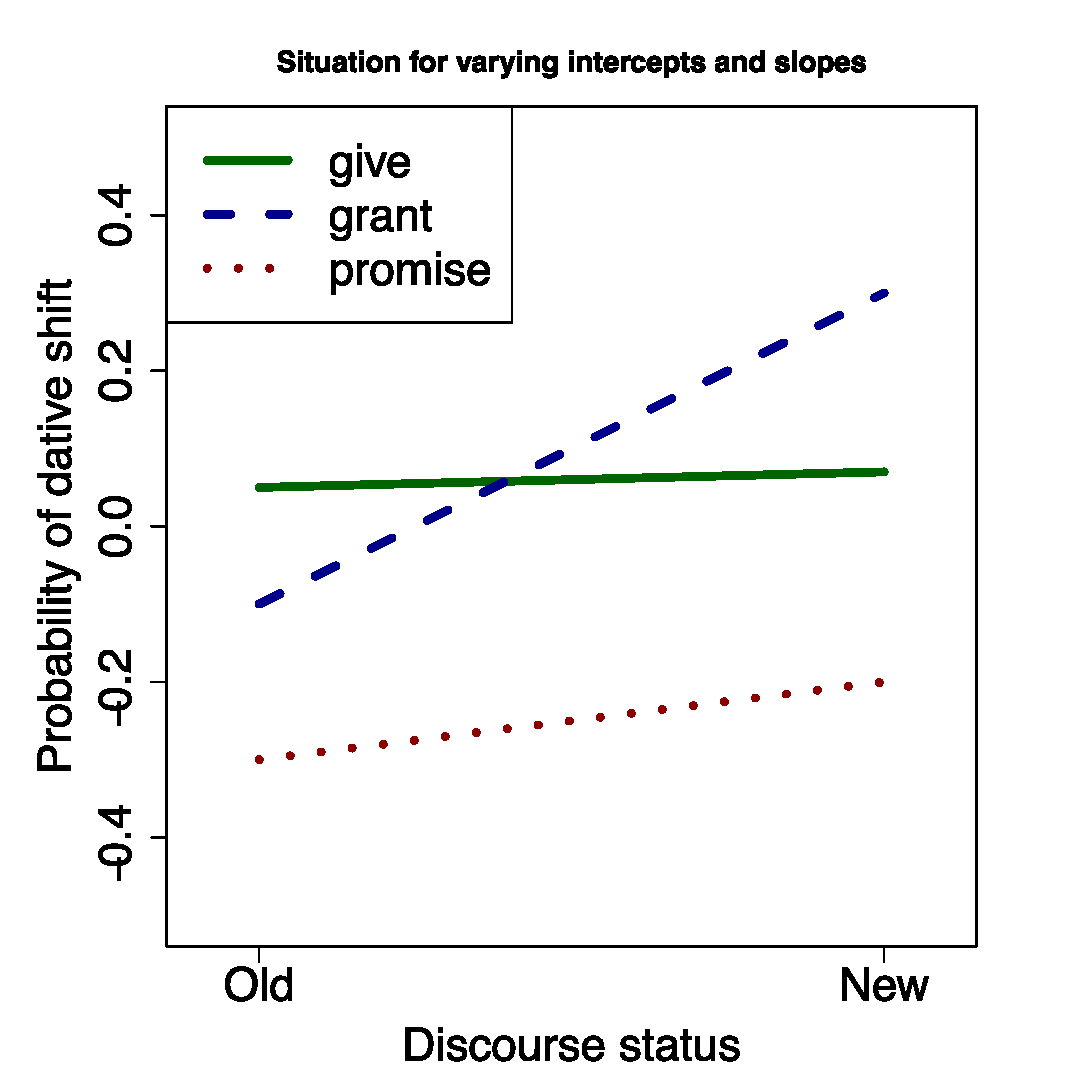
\includegraphics[width=0.5\textwidth]{graphics/var_int_slope}
  \caption{Illustration of data in situations for varying intercepts or varying intercepts and additional varying slopes}
  \label{fig:varintlsope}
\end{figure}

For the sake of the argument, we assume that we are looking at an alternation phenomenon like the dative alternation, wherein we are interested in the probability that, under given circumstances, the dative shift construction is chosen.
Looking at data set, it turns out that the probability of the dative shift changes for \textit{old} and \textit{new} dative NPs.
The verb lemma -- a typical candidate to be used as a random effect -- also influences the probability of either variant being used.
The situation can now be as in the left or the right panel of Figure~\ref{fig:varintlsope}.
In the situation illustrated in the left panel, the overall level in probability changes with the verb lemma, but for each verb lemma, the values change roughly accordingly in exemplars with old and new dative NPs.
Note that the lines are not perfectly parallel because the figure is supposed to be an illustration of a data set rather than a fitted model, and we always expect some chance variation in data sets.
In the situation depicted in the right panel, however, the overall levels are different between lemmas, but the lemma-specific tendencies also vary between exemplars with old and new NPs.
This is actually nothing but an interaction between two factors (verb lemma and discourse status).
However, if the verb lemma factor is used as a random effect grouping factor, the interaction is modeled as a so-called \textit{random slope}.
In the next section, it is shown how all the different types of data sets discussed so far can be modeled using fixed effects models or, alternatively, using mixed effects.
Which one is more appropriate will be argued to be better understood as a technical rather than a conceptual question.

\subsection{Model specification}
\label{sec:modelspecification}

In this section, it is discussed how the specification of mixed models differs from that of fixed effects models, and that for each model with random effects there is an alternative models with only fixed effects.
A major focus is on the question of when to use fixed and random effects.
The amount of technicality and notation is kept at the absolute minimum, but a few notational conventions are introduced as the absolute minimum required to understand both the output of lme4 and other packages in R as well as the literature on mixed models.
To make successful \textit{practical} use of mixed models, some level of fundamental understanding is required.
This section is based mostly on Part 2A of \citet{GelmanHill2006} (pp.~235--342).

\subsubsection{Simple random intercepts}

Readers with experience in fixed effects modeling (see the previous chapter in this handbook) should see that a grouping factor encoding the verb lemma, the speaker, the mode, the genre corresponding to a corpus exemplar (and all the other grouping factors discussed in the previous sections) could be specified as a normal fixed effect in a GLM.
In such a case, each of the $m$ levels of the speaker factor is dummy-coded, and for all but one of these binary dummy variables, a coefficient is estimated.
Logistic regression examples are used throughout this section, and we begin with the fictional corpus study of the dative alternation introduced in Sections~\ref{sec:hierarchicalormultilevelmodels} and \ref{sec:randominterceptsandslopes}.
We first specify a minimal model with only the dummies of the lemma grouping factor and one other (binary) predictor, namely discourse status.
There are $m$ verb lemmas (\ie groups) and $n$ observations.
As index variables, we use $j$ for groups and $i$ for observations.
In general, $\alpha$ is used for intercepts and $\beta$ for coefficients.
A specification of such a model is given in (\ref{eq:glm01}).

\begin{equation}
  Pr(y^i=1)=logit^{-1}(\alpha_0+\beta_d\cdot x_{d}^i+\beta_{l_1}\cdot x_{l_1}^i+\beta_{l_2}\cdot x_{l_2}^i+\cdots+\beta_{l_{m-1}}\cdot x_{l_{m-1}}^i)
  \label{eq:glm01}
\end{equation}

This models the estimate of the probability ($Pr$) that in observation $i$, the outcome variable $y^i$ is $1$, \ie that dative shift occurs.
$\alpha_0$ is the intercept, $\beta_d$ is the coefficient for the effect of discourse status.
$x_d^i$ is the value of the variable that encodes the discourse status for exemplar $i$ ($0$ for discourse-old NPs and $1$ for discourse-new NPs).
Furthermore, $\beta_{l_j}$ are the coefficients for the lemma dummy variables.
Finally, $x_{l_j}^i$ is the value ($0$ or $1$) for lemma $j$ in observation $i$.
If in exemplar $64$, the lemma is \textit{give} and \textit{give} is encoded as group $12$, then $i=64$, $j=12$, and $x_{l_{12}}^{64}=1$, whereas all $x_{l_j}^{64}=0$ with $j\neq12$.
Because one verb lemma dummy variable is on the intercept $\alpha_0$ and thus used as a reference, we only estimate $m-1$ instead of $m$ coefficients, \ie $j=1,\cdots,m-1$.%
\footnote{Picking one dummy as a reference level is necessary because otherwise infinitely many equivalent estimates of the model coefficients exist because one could simply add a constant to the intercept and subtract it from the dummies.
However, the estimator works under the assumption that there is a unique maximum likelihood estimate for the coefficient matrix.}
The function $logit^{-1}$ is the \textit{link function}, and its argument is the \textit{linear term} of the model.
It is obvious that in such a model, the effect of each verb lemma is treated as a fixed population parameter, exactly the same as the effect of discourse status.
The coefficient $\beta_d$ is estimated in exactly the same way as each $\beta_{l_j}$.

If we treat the same grouping factor as a random intercept, we let the intercept vary by group, and we give the varying intercepts a distribution instead of estimating $m-1$ coefficients.
This is the only relevant difference between a fixed effect and a random effect.
The model specification then looks like in (\ref{eq:glmm01}).

\begin{equation}
  P(y^i=1)=logit^{-1}(\alpha_{l}^{j[i]}+\beta_d\cdot x_d^i)
  \label{eq:glmm01}
\end{equation}

We now have an intercept $\alpha_l^{j[i]}$ that varies by group (instead of one term with its own coefficient per group).
We use the notation $\alpha_l^{j[i]}$ (borrowed in a modified form from \citealt{GelmanHill2006}) to indicate that the correct $j$-th lemma intercept is chosen for the $i$-th observation.
For example, if in exemplar $64$, the lemma is \textit{give}, which is group $12$, then $i=64$ and $j[64]=12$ (\ie the group appropriate for exemplar $64$ is group $12$), and $\alpha_l^{j[64]}=\alpha_l^{12}$.
The term $\beta_d\cdot x_d^i$ for the effect of discourse status remains unchanged when going from (\ref{eq:glm01}) to (\ref{eq:glmm01}).
Crucially, instead of estimating a batch of coefficients for the lemma effect, $\alpha_l$ is itself modeled, and random terms are predicted for each level of the grouping factor.
For this, the assumption in (\ref{eq:glmm02}) is made.

\begin{equation}
  \alpha_l^j\sim N(\mu_l,\sigma_l^2)
  \label{eq:glmm02}
\end{equation}

This is standard notation to indicate that the values of $\alpha_l^j$ follow a normal distribution with mean $\mu_l$ and a variance of $\sigma_l^2$.
In fact, we can regard (\ref{eq:glmm02}) as a minimal second-level model already, although one which simply predicts varying intercepts from a normal distribution.
All more complex models to be discussed below are extensions of this approach.
In the next section, the consequences of going from a fixed effect to a random effect are discussed.

\subsubsection{Choosing between random and fixed effects}
\label{sec:choosingbetweenrandomandfixedeffects}

There are primarily two points to consider which influence the decision to use random effects.
First, the variance in the intercepts (and for random intercept-random slope models also the covariance between intercepts and slopes) needs to be estimated.
Second, the random intercepts can be understood as a compromise between fitting separate models for each group of the grouping factor (\textit{no pooling}) and fitting a model while ignoring the grouping factor altogether (\textit{complete pooling}), see \citet[Ch.~12]{GelmanHill2006}.
While all conditions which were discussed in the previous chapter (independence of observations, non-collinearity, etc.) must also be met by hierarchical models, these two points add additional conditions.

As was stated above in (\ref{eq:glmm02}), the random intercepts are assumed to follow a normal distribution, and the variance $\sigma_l^2$ needs to be estimated with sufficient precision.
From the estimated variance and the data, the estimator then predicts the \textit{conditional modes} in GLMMs (\textit{conditional means} in LMMs) for each group (see \citealt[Ch.~1]{Bates2010}), which is the numerical value which software packages like lme4 produce, and these values are sometimes sloppily called ``random effects'' by practitioners.
This procedure, however, requires that the number of groups must not be too low to effectively achieve this.
As a rule of thumb, fewer than five levels means that a grouping factor should be included as a fixed effect, regardless of its conceptual nature.
Even if there is a default recommendation to use a speaker grouping variable as a random effect, it is ill-advised to do so if there are exemplars from less than five speakers in the sample.
Very often, the estimator will fail anyway under such conditions.
At the same time, the estimation of coefficients for a (dummy-coded) fixed effect becomes less precise and feasible with large numbers of levels, and at a certain point, a random effect might be the better or only option for technical reasons.

If, however, the number of groups is reasonably large, the next thing to consider is the number of observations per group.
As mentioned at the outset of this section, alternatives to using a random effect would be to estimate a separate model for each level of the grouping factor, or to include it as a fixed effect.
In both cases the effects are not treated as random variables, and fixed values per group are estimated without taking the between-group variance into account.
The conditional modes are \textit{shrunken} towards the overall intercept as a result (an effect called \textit{shrinkage}), and they tend to be more leveled compared to fixed effects estimates.
This effect becomes considerably weaker with larger per-group sample sizes.
With relatively low numbers of observations per group, on the other hand, fixed effect estimates tend to become inexact and will probably be dismissed because of growing uncertainty in the estimate (large confidence intervals, non-significance).
In this case, the conditional modes (or means) of random intercepts will just be shrunken more towards the overall intercept.
This considered, including a grouping factor as a random effect might be the only way of using it at all when the estimation as a fixed effect fails.

This section closes with an illustration.%
\footnote{The code for these and other simulations is available under a Creative Commons Attribution license: \url{https://github.com/rsling/Rstuff/tree/master/simulations/glmm}}
For this, 1,000 data sets were simulated which corresponded to the model in (\ref{eq:glmm03}) and (\ref{eq:glmm04}).
We drop the subscripts on $\alpha$, $\beta$, and $\mu$ for convenience since there is only one random intercept.

\begin{align}
  P(y^i=1) & =logit^{-1}(\alpha^{j[i]}+\beta_1\cdot x_1^i+\beta_2^i\cdot x_2^i)
  \label{eq:glmm03}\\
  \alpha^j & \sim N(\mu, \sigma)\label{eq:glmm04}
\end{align}

Again, this could be a model of a binary alternation.
$x_1$ was a binary variable (such as singular\slash plural) and $x_2$ a continuous variable (such as the length of the construction).
Since the data were simulated, the parameters to be estimated were known: $\beta_1=0.8$, $\beta_2=-1.3$, $\mu=0$, $\sigma=1.5$.
The number of groups was set to $5$ (the recommended minimum), the simulated values of the grouping factor were identical in each simulation, and there were $20$ observations per group.
Figure~\ref{fig:glmmj5i20} shows the distribution of the group levels based on the conditional modes predicted of all but the first group in the $1,000$ simulations.
Figure~\ref{fig:glmj5i20} shows the group estimates from a model where the grouping factor was added as a fixed effect.%
\footnote{The plots do not show the distribution of the raw conditional modes and coefficient estimates of the fixed effects.
Rather, the overall intercept was taken into account, and the plots thus show the distribution of the per-group prediction of the models, taking only the grouping factor into account.
This is what was pre-specified in the simulations.}

\begin{figure}[!htpb]
  \centering
  \includegraphics[width=0.6\textwidth]{graphics/glmmj5i20}
  \caption{Group levels in sample GLMM based on predicted random effect (conditional mode); 5 groups; 20 observations per group; 1,000 simulations; the horizontal line marks the true value}
  \label{fig:glmmj5i20}
\end{figure}
\begin{figure}[!htpb]
  \centering
  \includegraphics[width=0.6\textwidth]{graphics/glmj5i20}
  \caption{Estimated fixed effects for the grouping factor in sample GLM; 5 groups; 20 observations per level of the grouping factor; 1,000 simulations; the horizontal line marks the true value}
  \label{fig:glmj5i20}
\end{figure}

The per-group predictions lean slightly towards $0$ in the GLMM (Figure~\ref{fig:glmmj5i20}), but the fixed effects estimates in the GLM are prone to massive misestimations (see the large spread and increased 95\% intervals).
Even with as few as five levels of a grouping factor, however, random and fixed effects lead to very similar results, albeit with different advantages and disadvantages.
A few more differences will be discussed in Sections~\ref{sec:significancetestingandcoefficientsofdetermination} and \ref{sec:morecomplexmodels}.

\subsubsection{Significance testing, model selection and coefficients of determination}
\label{sec:significancetestingandcoefficientsofdetermination}

One commonly given reason to use a random effect is that ``the researchers are not interested in the individual levels of the random effect factor'' (or variations thereof).
Such recommendations should be taken with a grain of salt.
\citet[245--247]{GelmanHill2006} summarise the diverging and partially contradicting recommendations for what should be a random effect along with their motivations.
They conclude that there is essentially no clean conceptual way of deciding what should be a random effect and what a fixed effect.
Here, a rather technical approach was therefore suggested; see Section~\ref{sec:choosingbetweenrandomandfixedeffects}.

Clearly, however, it is not adequate to do any kind of significance test on the levels of the random effect factor, as is customary for fixed effects.
The conditional modes are not estimates, and only for estimates is significance testing a well-defined activity.
There are ways of calculating confidence intervals for conditional modes (see Section~\ref{sec:usinglme4}), but they should not be misused for talking about significance.
If this is absolutely required, fixed effects are the way to go.
Not doing significance tests for single levels of the grouping factor does, however, not mean that the researcher is not interested in the individual conditional modes, which is proven by the fact that they are often reproduced in research papers, for example in the form of a dot plot.
Additionally, a random effect allows the researcher to quantify the between-group variance, which is not possible in the same way with fixed effects.

A related question is \textit{model selection}, \ie whether the inclusion of the random effect improves the model quality.
First, the between-group variance should be checked.
If it is close to $0$, there is most likely not much going on between groups, or there simply was not enough data to estimate the variance.
In LMMs, it is possible to compare the residual (observation-level) variance with the between-group variance to see which one is larger, and to which degree.
If, for example, the residual variance is $\sigma_{\epsilon}=0.2$ and the between-group variance is $\sigma_{\alpha}=0.8$, then we can say that the between-group variance is four times larger than the residual variance, which would indicate a high importance of the random effect.
This comparison is impossible in GLMMs because their (several types of) residuals do not have the same straightforward interpretation as in LMMs.

Traditional model selection for random effects can be achieved through a likelihood ratio (LR) test comparing a model including the random effect and a model not including it.
Such pairs of models, where one is strictly a simplification of the other, are called \textit{nested models} (not to be confused with \textit{nested effects} discussed in Section~\ref{sec:crossedandnestedeffects}).
A much more robust option uses a parametric bootstrap replacements for the LR test (see Section~\ref{sec:usinglme4}).
It is \textit{not} appropriate to compare a model with a random effect and a model with the same factor as a fixed effect using \textit{any} test or metric (including information criteria).

Coefficients of determination (pseudo-$R^2$) should not be used for model selection, because they usually do not penalize complexity enough (\ie the pseudo-$R^2$ measures rise with added complexity).
They can still be used to give some idea of the model fit, however.
For GLMMs, \citet{NakagawaSchielzeth2013} have proposed a method that distinguishes between \textit{marginal} $R^2$ (fixed-effects-only) and \textit{conditional} $R^2$ (including random effects).
This has become a de facto standard, and we now show its consistency with Nagelkerke's $R^2$ for GLMs.
Using the simulations described in the last section, Figures~\ref{fig:rsqglmmj5i20} and \ref{fig:rsqglmj5i20} show that the marginal $R^2$ is roughly the same as Nagelkerke's $R^2$ in a GLM which ignores the grouping factor, and the conditional $R^2$ is roughly the same as Nagelkerke's $R^2$ in a GLM which includes the grouping factor as a fixed effect, given that the estimators converge for all these three types of models.

\begin{figure}[!htpb]
  \centering
  \includegraphics[width=0.6\textwidth]{graphics/rsqglmmj5i20}
  \caption{Distribution of Nakagawa \& Schielzeth's $R^2$ in the simulations described in Section~\ref{sec:choosingbetweenrandomandfixedeffects}}
  \label{fig:rsqglmmj5i20}
\end{figure}

\begin{figure}[!htpb]
  \centering
  \includegraphics[width=0.6\textwidth]{graphics/rsqglmj5i20}
  \caption{Nagelkerke's $R^2$ in the simulations described in Section~\ref{sec:choosingbetweenrandomandfixedeffects} for a GLM that ignores the grouping factor and a model that includes it as a fixed effect}
  \label{fig:rsqglmj5i20}
\end{figure}

Finally, it should be mentioned that adding a random intercept does not change the estimates nor the inferences (p-values) for fixed effects, at least if the grouping factor and the fixed effect are independent.
Figure~\ref{fig:pcomparison} compares the p-values obtained for the two fixed effects in the $1,000$ simulations described above for the GLMM and the GLM ignoring the grouping factor.
Notice that the $\beta_2$ effect has the higher effect strength, and p-values are generally lower.
If fixed effects and random effects are not independent, adding a varying slope should be considered, which is described in Section~\ref{sec:morecomplexmodels}.

\begin{figure}[!htpb]
  \centering
  \includegraphics[width=0.8\textwidth]{graphics/pcomparison}
  \caption{Comparison between the p-values of the fixed effects in the simulations described in Section~\ref{sec:choosingbetweenrandomandfixedeffects} for the GLMM and the GLM ignoring the grouping factor; the line was drawn using LOWESS (locally weighted scatterplot smoothing); the axes between the left and the right panel are on a different scale}
  \label{fig:pcomparison}
\end{figure}

\subsubsection{More complex models}
\label{sec:morecomplexmodels}

This section shows briefly how more complex models are specified before Section~\ref{sec:usinglme4} demonstrated how all models discussed are estimated in R, including interpretations of the output.

\paragraph{Varying intercepts and slopes}

A varying slope is an interaction between a fixed effect and a random effect, see Section~\ref{sec:randominterceptsandslopes}.
While it is possible to have just a varying slope, this is rarely useful, and we discuss only varying-intercept and varying-slope (VIVS) models.
We extend the simple model from (\ref{eq:glmm01}), and the fixed effect coefficients for which a random slope is specified simply receive group indices; see (\ref{eq:glmm05}).
Put simply, instead of a fixed coefficient, coefficients are predicted and assumed to come from a random (normal) distribution.
We use $\beta_{d:l}$ to denote the coefficient for discourse status varying by lemma.

\begin{equation}
  P(y^i=1)=logit^{-1}(\alpha_{l}^{j[i]}+\beta_{d:l}^{j[i]}\cdot x_d^i)
  \label{eq:glmm05}
\end{equation}

A source of problems in VIVS models is the fact that in addition to the variance in the intercepts and slopes, the covariance between them has to be estimated.
If in groups with a higher-than-average intercept, the slope is also higher than average, they are positively correlated, and vice versa.
These relations are captured in the covariance.
Therefore, condition (\ref{eq:glmm06}) is added, where the indices $l$ and $d:l$ are omitted for readability.

\begin{equation} 
  \left( \begin{smallmatrix} \alpha^j \\ \beta^j \end{smallmatrix}\right) \sim
    \left(
    \left( \begin{smallmatrix} \mu_{\alpha}\vphantom{\beta^j} \\ \mu_{\beta}\vphantom{\beta^j} \end{smallmatrix} \right), 
      \left( \begin{smallmatrix} \sigma_{\alpha}^2 & \rho\sigma_{\alpha}\sigma_{\beta} \\
	\rho\sigma_{\alpha}\sigma_{\beta} & \sigma_{\beta}^2 \end{smallmatrix} \right)
    \right)
  \label{eq:glmm06}
\end{equation}

(\ref{eq:glmm06}) says that the joint distribution of the intercepts $\alpha^j$ and the slopes $\beta^j$ follow a bivariate normal distribution with means $\mu_{\alpha}$ and $\mu_{\beta}$.
The variance in the intercepts is $\sigma_{\alpha}$, the variance in the slopes is $\sigma_{\beta}$, and the covariance between them is $\rho$.
Figure~\ref{fig:multnorm} shows the bivariate density distributions for two (1) negatively correlated, (2) non-correlated, and (3) positively correlated normally distributed variables.

\begin{figure}[!htpb]
  \centering
  \includegraphics[width=0.33\textwidth]{graphics/multnorm1}~\includegraphics[width=0.33\textwidth]{graphics/multnorm2}~\includegraphics[width=0.33\textwidth]{graphics/multnorm3}
  \caption{Bivariate normal density distribution with different correlation strengths ($\rho$); $\sigma_{\alpha}=\sigma_{\beta}=3$; $\mu_{\alpha}=\mu_{\beta}=0$}
  \label{fig:multnorm}
\end{figure}

Importantly, the number of parameters to estimate obviously increases with more complex model specifications, and the estimation of the parameters in the presence of complex variance-covariance matrices requires considerably more data than estimating a single variance parameter.
The estimator might converge, but typically covariance estimates of $-1$ or $1$ indicate that the data was too sparse for a successful estimation of the parameter.
In this case, the model is \textit{over-parametrized} and needs to be simplified.
In Section~\ref{sec:usinglme4}, it will be shown how to interpret the lme4 output appropriately.

\paragraph{Nested and crossed random effects}

As it was explained in Section~\ref{sec:crossedandnestedeffects}, nested random effects are adequate when grouping factors are nested within other grouping factors.
Technically, while varying slopes can be understood as interactions between a fixed and a random effect, nested random intercepts ca be understood interactions between two or more random effects.
Crossed random effects are just several unrelated random effects.
In the case of crossed and nested random intercepts, there are just more than one random intercept.
(\ref{eq:glmm07}) shows the model specification, extending (\ref{eq:glmm01}) with a varying intercept $\alpha_c$.
This could be for example semantic classes which nest individual lemmas.
It could also be another grouping factor for speaker, completely unrelated to the lemmas.

\begin{equation}
  P(y^i=1)=logit^{-1}(\alpha_{s}^{k[i]}+\alpha_{l}^{j[i]}+\beta_d\cdot x_d^i)
  \label{eq:glmm07}
\end{equation}

The difference is that in the nested case, $k[i]=k[j]$, \ie the level of the nesting factor can be selected based on the nested factor as well as based on the single observation.
In the crossed case, this is not the case.
As was mentioned in Section~\ref{sec:crossedandnestedeffects}, the questions is rather one of how the way the data are organised.
In the model specification (including model specification in R), there is not much to consider.

\paragraph{Second-level predictors}

In Section~\ref{sec:hierarchicalormultilevelmodels}, situations were introduced where the random effects themselves can be (partially) predicted from fixed-effects.
In this case, an additional linear model is specified for the random effect instead of the simple normal distribution predictor.
We extend (\ref{eq:glmm01}) by a predictor $\gamma_f$ for the lemma frequency.
The lemma frequencies themselves, we denote by $u_f$, and we index them with $j$, just like the verb lemmas.
This is reasonable because for each verb lemma, there is exactly one frequency.
The first-level model specification remains the same, namely (\ref{eq:glmm08}).

\begin{equation}
  P(y^i=1)=logit^{-1}(\alpha_{l}^{j[i]}+\beta_d\cdot x_d^i)
  \label{eq:glmm08}
\end{equation}

However, instead of (\ref{eq:glmm02}), the varying intercept is predicted from (\ref{eq:glmm09}).

\begin{equation}
  \alpha_l^j\sim N(\gamma_0+\gamma_f\cdot u_j^j,\sigma_l^2)
  \label{eq:glmm09}
\end{equation}

Instead of just the mean of the $\alpha_j$ values, the model in (\ref{eq:glmm09}) specifies a second-level intercept $\gamma_0$ and a second-level fixed coefficient $\gamma_f$.
If the lemma frequency plays a role, this approach can lead to a more precise prediction of the varying first-level intercept compared to the less elaborate approach in (\ref{eq:glmm02}).
True multilevel models increase the complexity of GLMMs, especially if third-level models, fourth-level models, etc. are used.
Situations for multilevel modeling are quite frequently encountered, however.
Especially when it comes to speakers as random effects, the age, the gender, the region of birth (if this grouping factor has too few levels to be used as a random effect nesting speakers), etc.\ are ideal second-level predictors.
The lme4 syntax treats second-level predictors like interactions between a fixed and a random effect, something which will be demonstrated in Section~\ref{sec:estimationofhierarchicalmodelsinr}.

% Readers finding it difficult to see why (\ref{eq:glmm09}) is a plain linear model could consider the equivalent formulation in (\ref{eq:glmm10}) and (\ref{eq:glmm11}).
% 
% \begin{align}
%   \alpha_l^j   =    & \gamma_0+\gamma_f\cdot u_j^j+\epsilon_l^j \label{eq:glmm10}\\
%   \epsilon_l^j \sim & N(0, \sigma^2) \label{eq:glmm11}
% \end{align}

% \paragraph{Remarks about models for time series}

\section{Packages and tools in R}
\label{sec:estimationofhierarchicalmodelsinr}

\subsection{Using lme4}
\label{sec:usinglme4}

This section focusses on lme4, the standard package to do multilevel modeling in R with maximum likelihood methods.
First, specifying models is discussed.
Second, it is shown how the output can be interpreted.

\paragraph{Specifying models}

Most important are the functions \texttt{lmer} and \texttt{glmer}, which extend the syntax of \texttt{lm} and \texttt{glm}.
The simple varying intercept model in \ref{eq:glmm01} looks as follows in R.
Informative variable names are used instead of Greek letters.

\vspace{0.5\baselineskip}

\pagebreak

\begin{lstlisting}[frame=trbl]
glmer(construction ~ discourse + (1 | lemma),
      family = binominal(link=logit), data = my.data)
\end{lstlisting}

The pipe operator \texttt{x|y} can be read as \textit{x varies by y}, and the intercept is denoted by \texttt{1}.
Therefore, \texttt{(1|lemma)} simply says that the intercept varies by lemma.

The VIVS model in (\ref{eq:glmm05}) would be specified as follows.
Only the formula is given from now on.

\vspace{0.5\baselineskip}

\begin{lstlisting}[frame=trbl]
construction ~ discourse + (1 + discourse | lemma)
\end{lstlisting}

In other words, before the pipe, the part of the model is repeated that should be modeled as varying by the grouping factor after the pipe.
If a varying slope is specified, the lemma is automatically also modeled as varying. 
The last formula can therefore be abbreviated to the following equivalent one.

\vspace{0.5\baselineskip}

\begin{lstlisting}[frame=trbl]
construction ~ discourse + (discourse | lemma)
\end{lstlisting}

In order to let \textit{only} the slope vary, the intercept has to be removed explicitly from the random part of the formula.

\vspace{0.5\baselineskip}

\begin{lstlisting}[frame=trbl]
construction ~ discourse + (discourse - 1 | lemma)
\end{lstlisting}

When there are more than one random effects, several bracketed terms can simply be added.
The following is the recommended specification for models like (\ref{eq:glmm07}), regardless of whether the effects are nested or crossed.

\vspace{0.5\baselineskip}

\begin{lstlisting}[frame=trbl]
construction ~ discourse + (1 + | lemma) +
               ( 1 | semantics )
\end{lstlisting}

Sometimes the recommendation is found to use the following notation for nested random effects, where \texttt{semantics} nests \texttt{lemma}.

\vspace{0.5\baselineskip}

\begin{lstlisting}[frame=trbl]
construction ~ discourse + ( 1 | semantics/lemma )
\end{lstlisting}

This is not necessary under normal circumstances.

\paragraph{Interpreting the output}

\subsection{Bootstrap methods for lme4}
\label{sec:bootstrapestimationforlme4}

%\subsection{Estimation using Markov-Chain Monte Carlo}
%\label{sec:estimationusingmarkovchainmontecarlo}
%
%\section{Representative studies}
%
%\subsection{STUDY 1}
%
%\subsubsection{Research questions}
%\subsubsection{Data}
%\subsubsection{Method}
%\subsubsection{Results}

\section{Further reading}
\label{sec:furtherreading}


\printbibliography

\end{document} 
